\documentclass{article}

\usepackage{microtype}
\usepackage{graphicx}
\usepackage{subcaption}
\usepackage{booktabs}
\usepackage{hyperref}
\usepackage{amsmath}
\usepackage{amssymb}
\usepackage{mathtools}
\usepackage{placeins}
\usepackage{tikz}
\usepackage{pgfplots}
\usepackage{multirow}
\pgfplotsset{compat=1.18}
\usetikzlibrary{arrows.meta,shapes.geometric,positioning,calc,fit,backgrounds}
\usepackage[capitalize,noabbrev]{cleveref}
\usepackage{icml2026}

\icmltitlerunning{Same-Evidence Reader-Budget Gating}

\begin{document}

\twocolumn[
\icmltitle{Same-Evidence Reader-Budget Gating for Token-Efficient Agent Memory}

\begin{icmlauthorlist}
\icmlauthor{Anonymous Authors}{anon}
\end{icmlauthorlist}
\icmlaffiliation{anon}{Anonymous Institution}
\icmlcorrespondingauthor{Anonymous Authors}{anonymous@example.com}
\icmlkeywords{agent memory, long-term memory, LLM agents, retrieval, token efficiency, efficient agents}

\vskip 0.3in
]

\printAffiliationsAndNotice{}

\begin{abstract}
Long-horizon agents can spend many reader tokens on redundant retrieved memories. We study a same-evidence reader-budget gate for the official open-source Mem0 package: the memory backend retrieves five records, and a deterministic risk rule chooses whether the frozen reader receives one or three of those exact records. On 311 LongMemEval questions, this adaptive gate answers 61/311 cases versus 62/311 for Mem0 top-5, while reducing reader tokens by 37.0\% and retrieved context tokens by 53.3\%. By comparison, fixed top-1 saves more tokens but falls to 50/311, fixed top-2 reaches 54/311, and fixed top-3 reaches 60/311. These results support a constrained token-savings claim for budgeted reader context, not a reproduction of Mem0 platform accuracy or a claim that the memory backend improves answer quality.
\end{abstract}

\section{Introduction}

Long-horizon agents increasingly depend on external memory to carry information across sessions, tools, and user interactions. Retrieval-centered memory systems are often evaluated by whether they recover useful evidence. A deployed frozen reader, however, also pays for every retrieved item it reads. Even when a memory backend retrieves relevant records, passing all of them to the reader can waste context on redundant, weakly relevant, or conflicting memories.

This paper asks a narrow token-budget question: under a fixed memory backend and frozen reader, how much of the retrieved evidence can be withheld before answer behavior changes? We keep the official open-source Mem0 package, reader model, prompt template, and decoding configuration fixed. The main intervention is not a new retriever. It is a same-evidence reader-budget gate that selects a smaller prefix of the exact Mem0 top-5 records already retrieved for the query.

We evaluate on LongMemEval~\cite{wu2025longmemeval}, a benchmark designed around long-term interactive memory, using the official Mem0 OSS package~\cite{chhikara2025mem0}. The completed run covers knowledge-update, single-session-preference, multi-session, and single-session-user, for 311 questions. Official Mem0 top-5 spends 151{,}558 reader tokens for 62 correct answers. A deterministic adaptive gate routes low-risk cases to top-1 evidence and high-risk cases to top-3 evidence using only revision markers and answer-like values in the Mem0 records. It spends 95{,}466 reader tokens for 61 correct answers. This is the central result: an exact same-evidence budget controller removes 37.0\% of reader tokens while changing the aggregate correct count by one case.

We also report ODV2-based secondary diagnostics because they motivated the budget-gating question. These are useful engineering checks, but the headline claim is deliberately based on the same-evidence adaptive gate because it avoids retrieval-overlap confounds. The result is not a benchmark-level Mem0 accuracy claim. It is a paired cost-reduction test under a constrained open-source Mem0 setup, and it preserves paired answer behavior rather than establishing high task quality: 244/311 cases are wrong for both top-5 and adaptive.

\paragraph{Contributions.}
We make three contributions. First, we define a same-evidence reader-budgeting interface that separates memory retrieval from the amount of retrieved evidence passed to a frozen reader. Second, we instantiate it for official Mem0 using a deterministic risk route over Mem0's own top-5 records. Third, we provide paired LongMemEval evidence showing large reader-context reductions, while explicitly treating accuracy as a guardrail and reporting fixed top-$k$, ODV2 compact, and ODV2-composed routes as secondary budget baselines.

\section{Related Work}

Retrieval-augmented generation shows that non-parametric memory can improve a frozen model by supplying external evidence~\cite{lewis2020rag}. Persistent-agent systems extend this idea to long-lived interaction. Generative Agents store observations and reflections~\cite{park2023generative}; MemGPT treats memory management as an operating-system-like problem~\cite{packer2023memgpt}; and Mem0 provides a scalable long-term memory substrate for production agents~\cite{chhikara2025mem0}. These systems make external memory a practical adaptation mechanism, but they do not fully separate evidence recall from evidence budgeting.

Long-term memory benchmarks make that distinction important. LoCoMo evaluates very long-term conversational memory~\cite{maharana2024locomo}, and LongMemEval focuses on interactive assistant memory across sessions~\cite{wu2025longmemeval}. Many failures in these settings arise because evidence changes over time or because multiple retrieved memories are only partially relevant. Our work treats revision and conflicting answer values as routing signals for reader-budget control, rather than claiming to solve memory consolidation.

This design is related to belief revision~\cite{alchourron1985logic}, but implemented as an engineering layer for LLM agents rather than a symbolic knowledge base. It is also aligned with efficient adaptation. Parameter-efficient tuning and continual-learning methods adapt model weights~\cite{hu2022lora,wang2024comprehensive}, whereas memory-state updates can be cheaper when the change is user-specific or short-lived. This is consistent with Green AI arguments for preferring lower-cost mechanisms when quality is preserved~\cite{strubell2019energy,schwartz2020green}.

\section{Method}

\subsection{Same-Evidence Reader-Budget Gate}

Let $B_5(q)=(r_1,\ldots,r_5)$ be the five records returned by official Mem0 OSS for query $q$. The reader-budget gate never changes this retrieved set and never injects records from another store. It only chooses how many of the ranked records to expose to the frozen reader. Fixed baselines are therefore
\begin{equation}
B_k(q)=(r_1,\ldots,r_k),\quad k\in\{1,2,3,4,5\}.
\end{equation}

The adaptive gate uses a deterministic risk rule over Mem0's own retrieved text. From the first four records, it counts revision markers such as \emph{currently}, \emph{recently}, \emph{changed}, \emph{updated}, and \emph{used to}. It also extracts answer-like values with a numeric regex that covers money, times, percentages, durations, distances, and other digit-bearing values. The route is high-risk if at least one revision marker is present or at least two distinct answer-like values are present. High-risk queries use $B_3(q)$; all other queries use $B_1(q)$:
\begin{equation}
B_{\textsc{adapt}}(q)=
\begin{cases}
B_3(q), & h(B_5(q))=1,\\
B_1(q), & h(B_5(q))=0.
\end{cases}
\end{equation}
This route uses no gold labels, predictions, category labels, or ODV2 records. It is a conservative reader-budget controller over a fixed retrieved evidence set.

\subsection{Secondary ODV2 Operating Points}

We also report two ODV2 diagnostics because they motivated the budget-gating question. The compact ODV2 wrapper uses the same OSS Mem0 package and local reader, returns at most two records, and applies a conservative stale-state guard. The guard fires rarely in the completed run. Artifact inspection also shows that ODV2's returned records are not always a subset of the corresponding official Mem0 top-5 records. We therefore treat ODV2 compact and the ODV2/top-3 composed route as secondary operating points, not as the causal basis for the same-evidence claim.

\section{Evaluation}

We evaluate on LongMemEval~\cite{wu2025longmemeval}. The baseline is \texttt{official\_mem0}, an adapter around the official open-source Mem0 package. The baseline retrieves five Mem0 records per query and passes all five to the frozen reader. We replay the same saved Mem0 records through the same reader using only the first $k \in \{1,2,3,4\}$ records, then compose \texttt{official\_mem0\_same\_evidence\_adaptive} by routing each case to the already computed top-1 or top-3 replay. These same-evidence replays do not rerun Mem0 extraction, retrieval, or ODV2 state maintenance. We report paired comparisons on four LongMemEval categories: knowledge-update ($N=78$), single-session-preference ($N=30$), multi-session ($N=133$), and single-session-user ($N=70$), for 311 total questions.

The Mem0 extraction LLM is \texttt{Qwen/Qwen2.5-7B-Instruct} served through vLLM with a 16k serving context, bfloat16 weights, add batch size 16, 2000 maximum message characters, and raw fallback disabled to avoid invalid empty-memory runs. The Mem0 embedder is \texttt{sentence-transformers/all-MiniLM-L6-v2} with local Qdrant storage. The frozen reader is also \texttt{Qwen/Qwen2.5-7B-Instruct}, evaluated with the repository local-Hugging Face backend, bfloat16 inference, inference batch size 64, reader flush size 8, and an 8192-token reader context window. Both policies use the same cleaned input file, \texttt{data/longmemeval\_s\_cleaned.json}, and the same reader prompt template.

Primary metrics are prompt tokens, reader total tokens, retrieved context tokens, and retrieved item count. Accuracy, paired wins, and paired losses against \texttt{official\_mem0} are reported as guardrail metrics to show how much answer behavior changes under budget reduction. Pairing is by LongMemEval case id, so a win means the budgeted policy is correct where the baseline is incorrect, and a loss means the reverse. Accuracy uses a local span-match proxy rather than the official leaderboard protocol: normalized exact match or normalized span match after lowercasing, article removal, punctuation removal, and whitespace normalization. The results therefore should not be compared directly to Mem0 platform or leaderboard numbers, which use different Mem0 backends, larger retrieval depths, and different evaluation harnesses~\cite{mem0benchmarks2026}.

For secondary context, we also report \texttt{official\_mem0\_odv2\_selective}, a compact ODV2 wrapper around the same OSS Mem0 setup, and \texttt{official\_mem0\_staleaware\_gate}, a post-hoc composition of ODV2 compact and top-3 replay. These rows are not the basis of the same-evidence claim because ODV2 retrieval is not guaranteed to overlap exactly with the baseline top-5. As a secondary latency sanity check, we run a cache-free reader-only replay on a deterministic 64-case subset shared by official Mem0 top-5, the same-evidence adaptive row, and fixed top-1, top-2, and top-3 rows. This replay disables the response cache and reuses already-retrieved records, so it checks that the token reduction is reflected in frozen-reader wall-clock time without rerunning Mem0 ingestion or extraction. Finally, we run an oracle answer-session replay on 64 cases by giving the reader only LongMemEval sessions marked as containing the answer.

\paragraph{Scope of the run.}
The experiment is intended as an efficiency ablation under a constrained OSS Mem0 reader budget, not as a reproduction of the published Mem0 platform result. The relevant question is paired: given the same OSS Mem0 extraction run and the same frozen reader, how much of the same retrieved context can be removed before accuracy changes? This design makes token savings directly interpretable, but it also explains the low absolute accuracy observed in the current run.

\section{Results}

\begin{table*}[t]
\caption{LongMemEval results for the exact same-evidence adaptive gate. $\Delta$Prompt is adaptive gate minus official Mem0 top-5. Wins are cases where the adaptive gate is correct and Mem0 top-5 is wrong; losses are the reverse. \texttt{Top2} is a fixed replay of the same Mem0 retrieved records with only the first two records passed to the reader.}
\label{tab:aggregate_results}
\vskip 0.15in
\begin{center}
\begin{small}
\begin{sc}
\begin{tabular}{lccccccc}
\toprule
Category & $N$ & Mem0 Acc & Adaptive Acc & Top2 Acc & $\Delta$Prompt & Win & Loss \\
\midrule
Knowledge-update & 78 & 25/78 (.321) & 25/78 (.321) & 23/78 (.295) & $-39.54\%$ & 1 & 1 \\
\midrule
Single-sess-pref & 30 & 0/30 (.000) & 1/30 (.033) & 0/30 (.000) & $-43.69\%$ & 1 & 0 \\
\midrule
Multi-session & 133 & 7/133 (.053) & 7/133 (.053) & 4/133 (.030) & $-39.32\%$ & 2 & 2 \\
\midrule
Single-sess-user & 70 & 30/70 (.429) & 28/70 (.400) & 27/70 (.386) & $-42.16\%$ & 1 & 3 \\
\midrule
Total & 311 & 62/311 (.199) & 61/311 (.196) & 54/311 (.174) & $-40.43\%$ & 5 & 6 \\
\bottomrule
\end{tabular}
\end{sc}
\end{small}
\end{center}
\vskip -0.1in
\end{table*}

\begin{table*}[t]
\caption{Efficiency over the exact official Mem0 evidence frontier. Reader-token changes are relative to official Mem0 top-5. The adaptive row selects only between official Mem0 top-1 and top-3 replays.}
\label{tab:token_budget}
\vskip 0.15in
\begin{center}
\begin{tiny}
\begin{sc}
\begin{tabular}{lccccc}
\toprule
Policy & Records & Correct & Reader tok. & $\Delta$ tok. & Tok./correct \\
\midrule
\texttt{top1} & 1 & 50/311 & 65{,}812 & $-56.58\%$ & 1{,}316 \\
\texttt{top2} & 2 & 54/311 & 86{,}002 & $-43.25\%$ & 1{,}593 \\
\texttt{adaptive} & 1/3 & 61/311 & 95{,}466 & $-37.01\%$ & 1{,}565 \\
\texttt{top3} & 3 & 60/311 & 110{,}058 & $-27.38\%$ & 1{,}834 \\
\texttt{top4} & 4 & 59/311 & 130{,}157 & $-14.12\%$ & 2{,}206 \\
\texttt{top5} & 5 & 62/311 & 151{,}558 & --- & 2{,}444 \\
\bottomrule
\end{tabular}
\end{sc}
\end{tiny}
\end{center}
\vskip -0.1in
\end{table*}

\begin{table}[t]
\caption{Mechanism and evidence-overlap audit. The headline adaptive gate uses only official Mem0 top-$k$ replay rows; ODV2 rows are secondary because their returned records can differ from the baseline top-5.}
\label{tab:mechanism_attribution}
\vskip 0.15in
\begin{center}
\begin{scriptsize}
\begin{sc}
\begin{tabular}{lr}
\toprule
Diagnostic & Count \\
\midrule
Same-evidence adaptive rows & 311 \\
Routes to Mem0 top-1 & 105 \\
Routes to Mem0 top-3 & 206 \\
Mem0 records omitted vs top-5 & 827 \\
ODV2 rows with outside-top-5 record & 63 \\
ODV2 records outside baseline top-5 & 111 \\
Stale records removed by ODV2 guard & 2 \\
\bottomrule
\end{tabular}
\end{sc}
\end{scriptsize}
\end{center}
\vskip -0.1in
\end{table}

\paragraph{Accuracy guardrail.}
Across the 311 paired cases, the automatic span scorer marks official Mem0 OSS top-5 correct on 62 cases and the same-evidence adaptive gate correct on 61 cases. The paired automatic difference is therefore one case, or $-0.3$ percentage points. There are 5 automatic paired wins for the adaptive gate and 6 automatic paired losses; 56 cases are correct for both methods and 244 are wrong for both. Because this one-case difference is sensitive to scorer boundary cases, we author-audited all 11 automatic disagreements and a deterministic 20-case agreement sample. The disagreement audit labels 5 cases correct for top-5 and 5 for adaptive, and the full 31-case worksheet labels both policies correct on 17 cases. The audit does not support an accuracy improvement claim, but it supports treating the automatic one-case difference as a guardrail rather than a substantive accuracy loss.

\paragraph{Reader-budget reduction.}
The token-savings signal is the central result. The adaptive gate reduces prompt tokens by 40.43\%, total reader tokens by 37.01\%, retrieved context tokens by 53.32\%, and retrieved items by 53.35\%. This is a clean same-evidence result: all reader inputs are prefixes of the exact Mem0 top-5 records used by the baseline. The ODV2 compact row remains useful as a secondary operating point, reducing reader tokens by 42.70\%, but it is not the main causal evidence because 63/311 ODV2 rows contain at least one record outside the corresponding official Mem0 top-5.

\paragraph{Cost-normalized utility.}
Because the goal is token savings under an accuracy guardrail, the most direct utility view is reader tokens spent per correct answer. Official Mem0 top-5 spends 151{,}558 reader tokens for 62 correct answers, or 2{,}444 reader tokens per correct answer. The same-evidence adaptive gate spends 95{,}466 reader tokens for 61 correct answers, or 1{,}565 tokens per correct answer. Equivalently, the top-5 baseline spends 56{,}092 additional reader tokens to recover one additional aggregate correct answer. Fixed top-1 has the lowest token cost per correct answer but answers only 50 cases correctly; fixed top-2 saves slightly more tokens than the adaptive gate but answers seven fewer cases correctly.

A paired bootstrap over 20{,}000 case resamples gives a 95\% interval of 35.5--38.5\% for the adaptive reader-token reduction and 28.5--42.7\% for tokens-per-correct reduction. The same bootstrap gives an accuracy-delta interval of $-2.57$ to $+1.61$ percentage points. We do not claim statistical non-inferiority for any budgeted row. The same-evidence adaptive result should be read as an accuracy-guarded operating point, not as an accuracy improvement.

\paragraph{Scorer sanity checks.}
The adaptive guardrail audit is the scorer check for the headline comparison. We also retain the earlier 50-case audit from the original ODV2 comparison only as secondary scorer context, not as evidence for the headline adaptive policy. That audit agrees with the automatic span scorer on 91/100 decisions across official Mem0 and ODV2 compact. Together, these checks support using the local span scorer as a rough guardrail, while preserving the paper's narrower claim: token savings under observed paired answer behavior, not statistically certified non-inferiority.

\begin{table}[t]
\caption{Sensitivity of the same-evidence adaptive rule. The default route uses candidate-$k=4$, revision threshold 1, and distinct-value threshold 2. All rows select only between official Mem0 top-1 and top-3 reader replays.}
\label{tab:adaptive_sensitivity}
\vskip 0.1in
\begin{center}
\begin{tiny}
\begin{tabular}{@{}lcccc@{}}
\toprule
Setting & Route 1/3 & Correct & Reader tok. & $\Delta$ \\
\midrule
Default & 105/206 & 61/311 & 95{,}466 & $-37.01\%$ \\
\midrule
Less & 137/174 & 60/311 & 91{,}039 & $-39.93\%$ \\
\midrule
More & 87/224 & 61/311 & 97{,}962 & $-35.36\%$ \\
\midrule
Value & 126/185 & 60/311 & 92{,}393 & $-39.04\%$ \\
\midrule
Broad & 70/241 & 61/311 & 100{,}415 & $-33.74\%$ \\
\bottomrule
\end{tabular}
\end{tiny}
\end{center}
\vskip -0.1in
\end{table}

All sensitivity rows are evaluated on the same completed run and should be read as robustness checks around the deterministic rule, not as evidence of pre-registered model selection.

\paragraph{Top-$k$ attribution baselines.}
\Cref{tab:token_budget,tab:mechanism_attribution} show that fixed truncation alone is not the whole story. Plain top-1 replay saves the most tokens but drops to 50/311 correct. Plain top-2 uses 86{,}002 total reader tokens but answers only 54/311 cases correctly. Plain top-3 recovers 60/311 correct answers, but pays 110{,}058 reader tokens. The adaptive gate lies between top-2 and top-3 in cost, answers one more case than top-3, and uses 14{,}592 fewer reader tokens than top-3. This is the strongest causal evidence in the paper because the compared prompts differ only in how many official Mem0 records the reader sees.

\paragraph{Absolute accuracy caveat.}
The absolute accuracy values are low, especially in single-session-preference and multi-session. This is not hidden in the result tables because it directly affects how the paper should be read. The experiment is a paired efficiency ablation under one constrained OSS Mem0 setup and one local reader, not a claim that either method reaches published Mem0 platform accuracy. The oracle answer-session sanity check reaches 27/64 correct (42.2\%) on its 64-case sample, including 10/12 single-session-user cases, showing that the same reader and scorer can solve substantially more cases when focused answer evidence is supplied. The oracle result remains far from saturated, so it should be read only as a sanity check on evidence availability and scorer strictness.

\paragraph{Uncertainty and latency sanity check.}
The paired accuracy differences are small relative to the number of cases, and we do not claim statistical non-inferiority. We keep reader-token count as the primary efficiency metric because it is deterministic from the generated prompts and directly controls hosted-reader cost. In the cache-free 64-case reader replay, official Mem0 top-5 takes 62.6 ms/case, while the same-evidence adaptive row takes 37.2 ms/case. Fixed top-1, top-2, and top-3 take 26.2, 33.4, and 39.6 ms/case, respectively. Adaptive answers 10/64 cases correctly on this subset versus 9/64 for top-5, top-2, and top-3; top-1 also answers 10/64. Peak allocated GPU memory is 16{,}179 MiB for top-5 and 15{,}686 MiB for adaptive. This is a reader-only latency sanity check over saved records, not a deployment benchmark; the present run still does not report energy or end-to-end wall-clock cost across heterogeneous hardware.

\begin{figure}[t]
\centering
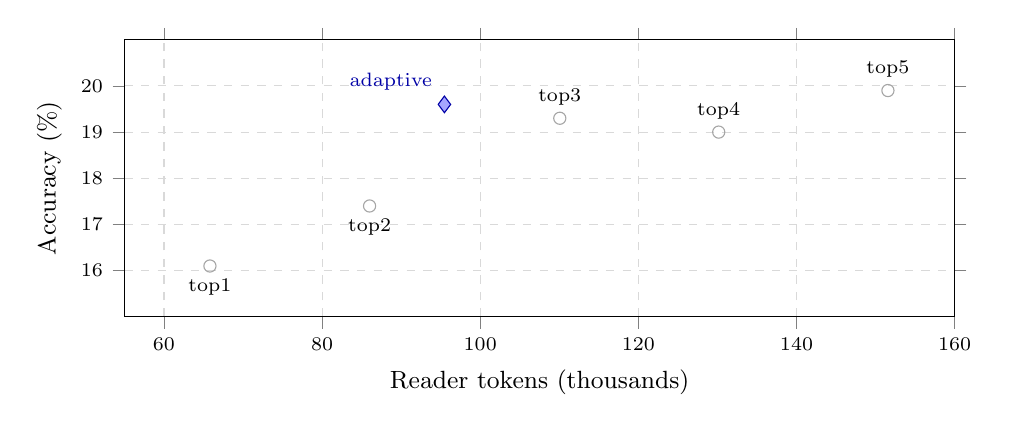
\begin{tikzpicture}
\begin{axis}[
    width=\columnwidth,
    height=5.1cm,
    xlabel={Reader tokens (thousands)},
    ylabel={Accuracy (\%)},
    xlabel style={font=\small},
    ylabel style={font=\small},
    xmin=55, xmax=160,
    ymin=15, ymax=21,
    xtick={60,80,100,120,140,160},
    ytick={16,17,18,19,20},
    xticklabel style={font=\scriptsize},
    yticklabel style={font=\scriptsize},
    grid=major, grid style={dashed, gray!30},
    tick align=outside,
    clip=false,
]
\addplot[only marks, mark=o, mark size=2.2pt, draw=gray!70, fill=gray!25]
coordinates {
    (65.812,16.1)
    (86.002,17.4)
    (110.058,19.3)
    (130.157,19.0)
    (151.558,19.9)
};
\addplot[only marks, mark=diamond*, mark size=3.0pt, draw=blue!65!black, fill=blue!35]
coordinates {(95.466,19.6)};
\node[font=\scriptsize, anchor=north, yshift=-1.2pt] at (axis cs:65.812,16.1) {top1};
\node[font=\scriptsize, anchor=north, yshift=-1.2pt] at (axis cs:86.002,17.4) {top2};
\node[font=\scriptsize, anchor=south east, xshift=-1.0pt, yshift=1.5pt, text=blue!65!black] at (axis cs:95.466,19.6) {adaptive};
\node[font=\scriptsize, anchor=south, yshift=1.2pt] at (axis cs:110.058,19.3) {top3};
\node[font=\scriptsize, anchor=south, yshift=1.2pt] at (axis cs:130.157,19.0) {top4};
\node[font=\scriptsize, anchor=south, yshift=1.2pt] at (axis cs:151.558,19.9) {top5};
\end{axis}
\end{tikzpicture}
\caption{Accuracy--cost tradeoff for exact official Mem0 evidence only. The blue marker is the same-evidence adaptive gate; gray markers are fixed Mem0 top-$k$ replays.}
\label{fig:token_reduction}
\end{figure}

\section{Discussion}

The current results support a narrower decomposition of agent memory into evidence recall and reader-budget control. Official Mem0 OSS supplies the retrieved evidence, while the same-evidence gate decides how much of that ranked evidence is passed to the frozen reader. The adaptive route substantially reduces the amount of text read by the answerer while staying within one aggregate correct answer of the top-5 baseline. This distinction should remain central to the paper framing.

This framing matters for cost-aware agent memory. If every memory query requires passing many retrieved facts to a reader, long-horizon agents inherit a growing prompt-cost burden even when the backend can retrieve relevant evidence. The reported run shows that a lightweight post-retrieval gate can remove over half of retrieved context tokens under a fixed open-source Mem0 setup. The adaptive gate is best used as a budgeted utility ablation: it reduces reader tokens per correct answer from 2{,}444 to 1{,}565, improves substantially over fixed top-1 and top-2 in accuracy, and uses fewer tokens than fixed top-3 while answering one more case correctly.

The low absolute accuracy is also informative. It indicates that this run is not a reproduction of the published Mem0 platform benchmark configuration. In our setup, official Mem0 OSS retrieves five records and the reader is a local Qwen-7B model scored by a strict local span-match proxy. Published Mem0 platform results use different infrastructure and much larger retrieval depths. The manual audit reinforces this interpretation: several wrong answers are better described as missing retrieved evidence than reader arithmetic failures. The proper comparison inside this paper is therefore paired and local: official Mem0 OSS top-5 versus smaller prefixes of the same retrieved Mem0 evidence.

\section{Limitations}

The main limitation is that the result does not show an accuracy improvement. Accuracy is not the target metric of the paper; it is a guardrail for the token-savings claim. We therefore do not claim that the adaptive gate beats Mem0, official Mem0, or the Mem0 platform on broad conversational QA. The defensible result is narrower: same-evidence adaptive gating is a lower-cost operating point that reduces reader tokens by 37.0\% and reader tokens per correct answer by 36.0\% relative to the top-5 official Mem0 baseline, while losing one aggregate correct answer.

Second, the baseline is the official open-source Mem0 package under a constrained retrieval budget, not the Mem0 managed platform and not the published top-50 or top-200 benchmark setting. The low absolute accuracy should be reported rather than hidden, but it should not be interpreted as a claim about Mem0 platform quality. The top-$k$ replay study covers $k \le 5$ from the completed run, but a stronger version should compare top-10, top-50, and top-200 retrieval to separate retrieval recall failures from reader failures.

Third, the adaptive route is deterministic but not pre-registered; it should be validated prospectively in a fresh run. It also composes existing top-1 and top-3 replay outputs rather than measuring a single online controller with its own retrieval path. The cache-free row measures reader latency for saved adaptive inputs, but not Mem0 retrieval time, routing overhead, or serving under concurrent traffic. A more complete ablation should compare online query-adaptive gates, simple deduplication, stale-state suppression without compaction, and compaction without stale-state suppression. Fourth, token count is a proxy for reader cost, not a complete deployment metric. This is appropriate for the paper's token-savings claim, but future deployment work should add repeated latency trials, GPU utilization, energy, and wall-clock cost. Finally, the current experiments are text-only. The SCALE setting motivates multimodal agent memory, but this paper only tests the text memory layer that a multimodal extraction system could feed.

\section{Conclusion}

Same-evidence adaptive gating provides evidence that agent memory systems can reduce frozen-reader token budgets without changing the memory backend. On 311 paired LongMemEval questions, the adaptive gate reduces reader total tokens by 37.0\% and retrieved context tokens by 53.3\%, while the accuracy guardrail changes from 19.9\% to 19.6\%. Fixed top-2 reaches a lower token budget but lower accuracy, 17.4\%, while fixed top-3 reaches 19.3\% at a larger budget. The main contribution is not a universal retriever or a new benchmark-leading memory system. It is a clean, same-evidence budget ablation showing that a frozen reader can often receive fewer retrieved memories while preserving most paired answer behavior in this constrained Mem0 OSS setup.

\section*{LLM/Agent Usage Disclosure}

LLM-based coding and writing tools were used to assist with implementation and reviewer-style critique. The authors remained responsible for experiment execution, numerical results, claim selection, and final manuscript content.

\section*{Artifact Status}

The submitted repository includes the official Mem0 package runner, top-$k$ replay, same-evidence adaptive composition, token analysis, submission-check generation, cache-free reader benchmarking, oracle answer-context replay, and per-case JSONL diagnostics. The active run directory is \path{results/official_mem0_basecompact_full_20260502T072459Z}. It contains the top-$k$ replay rows, adaptive rows, cleaned-input checksum, command logs, vLLM/server diagnostics, and GPU snapshots. Submission-check outputs include the adaptive guardrail audit, reviewed 50-case scorer audit, oracle answer-context rows, and cache-free reader traces.

\section*{Reproducibility Commands}

The adaptive rows are regenerated with \path{scripts/compose_official_mem0_same_evidence_adaptive.py}; the route uses candidate-$k=4$, revision-signal threshold 1, and distinct-value threshold 2. The paper tables are regenerated from per-case JSONL outputs using the repository scripts named above. The completed run stores command logs, diagnostics, top-$k$ replays, bootstrap summaries, adaptive guardrail audit, manual-audit sample, cache-free reader benchmark, and oracle answer-context replay under the active result directory.

\FloatBarrier
\bibliographystyle{icml2026}
\bibliography{references}

\end{document}
